% Modelo de monografia criado para a Faculdade de Computação
% da Universidade Federal do Pará a partir da classe abntex2.
% Este documento só deverá ser alterado para incluir ou excluir
% elementos pré e pós textuais. Use o comentário do latex (%) caso
% deseje excluir algum elemento.

%% abtex2-modelo-trabalho-academico.tex, v-1.9.6 laurocesar
%% Copyright 2012-2016 by abnTeX2 group at http://www.abntex.net.br/ 
%%
%% This work may be distributed and/or modified under the
%% conditions of the LaTeX Project Public License, either version 1.3
%% of this license or (at your option) any later version.
%% The latest version of this license is in
%%   http://www.latex-project.org/lppl.txt
%% and version 1.3 or later is part of all distributions of LaTeX
%% version 2005/12/01 or later.
%%
%% This work has the LPPL maintenance status `maintained'.
%% 
%% The Current Maintainer of this work is the abnTeX2 team, led
%% by Lauro César Araujo. Further information are available on 
%% http://www.abntex.net.br/
%%
%% This work consists of the files abntex2-modelo-trabalho-academico.tex,
%% abntex2-modelo-include-comandos and abntex2-modelo-references.bib
%%

% ------------------------------------------------------------------------
% ------------------------------------------------------------------------
% abnTeX2: Modelo de Trabalho Academico (tese de doutorado, dissertacao de
% mestrado e trabalhos monograficos em geral) em conformidade com 
% ABNT NBR 14724:2011: Informacao e documentacao - Trabalhos academicos -
% Apresentacao
% ------------------------------------------------------------------------
% ------------------------------------------------------------------------

\documentclass[
	% -- opções da classe memoir --
	12pt,				% tamanho da fonte
	openright,			% capítulos começam em pág ímpar (insere página vazia caso preciso)
	oneside,			% para impressão em frente e verso. Oposto a oneside
	a4paper,			% tamanho do papel.
	% -- opções da classe abntex2 --
	chapter=TITLE,		% títulos de capítulos convertidos em letras maiúsculas
	%section=TITLE,		% títulos de seções convertidos em letras maiúsculas
	%subsection=TITLE,	% títulos de subseções convertidos em letras maiúsculas
	%subsubsection=TITLE,% títulos de subsubseções convertidos em letras maiúsculas
	% -- opções do pacote babel --
	english,			% idioma adicional para hifenização
	french,				% idioma adicional para hifenização
	spanish,			% idioma adicional para hifenização
	brazil				% o último idioma é o principal do documento
	]{abntex2}

% ---
% Pacotes básicos 
% ---
\usepackage{lmodern}			% Usa a fonte Latin Modern
\usepackage{mathptmx}			% Usa a fonte Times New Roman
\usepackage[T1]{fontenc}		% Selecao de codigos de fonte.
\usepackage[utf8]{inputenc}		% Codificacao do documento (conversão automática dos acentos)
\usepackage{lastpage}			% Usado pela Ficha catalográfica
\usepackage{indentfirst}		% Indenta o primeiro parágrafo de cada seção.
\usepackage{color}				% Controle das cores
\usepackage{graphicx}			% Inclusão de gráficos
\usepackage{subcaption}			% Inclusão de gráficos lado a lado
\usepackage{microtype} 			% para melhorias de justificação
\usepackage{tabularx,ragged2e}	% Para inserir tabelas
\usepackage{multirow}			% Para mesclar células
\usepackage[dvipsnames,table,xcdraw]{xcolor}		% Permite adicionar cores nas linhas de tabelas
\usepackage{fancyvrb}			% Permite adicionar arquivos de texto
\usepackage[portuguese, ruled, linesnumbered]{algorithm2e} % Uso de algoritmos
\usepackage{amsfonts}			% Permite usar notação de conjuntos
\usepackage{amsmath}			% Permite citar equações
\usepackage{amsthm}				% Permite criar teoremas e experimentos
\usepackage[font={bf, small}, labelsep=endash, labelfont=bf]{caption}	% Faz legenda de figuras ficarem em negrito
\usepackage{cancel}				% Permite fazer expressão tendendo a zero
\usepackage{epstopdf}			% Converte eps para pdf
\usepackage[final]{pdfpages}

\newcolumntype{L}{>{\RaggedRight\arraybackslash}X}
% ---
		
% ---
% Pacotes adicionais, usados apenas no âmbito do Modelo Canônico do abnteX2
% ---
\usepackage{lipsum}				% para geração de dummy text
% ---

% ---
% Pacotes de citações
% ---
%\usepackage[brazilian,hyperpageref]{backref}	 % Paginas com as citações na bibl
\usepackage[alf, abnt-emphasize=bf]{abntex2cite}	% Citações padrão ABNT

% ---
% Customizações para o layout da UFPA
% ---
\usepackage{modelo-ufpa/ufpa}
\usepackage{float}
% Muda o título de lista de ilustrações para lista de figuras
\addto\captionsbrazil{%
  \renewcommand{\listfigurename}%
    {Lista de Ilustrações}%
	\renewcommand{\listtablename}%
    {Lista de Tabelas}%
}

% Permite utilizar figuras sem precisar colocar o caminho absoluto
\graphicspath{{imagens/}}

% Define o ambiente de experimentos
\theoremstyle{definition}
\newtheorem{experimento}{Experimento}[section]
\newcommand{\experimentoautorefname}{Experimento}

%sem cabeçalho 
% --- 
% CONFIGURAÇÕES DE PACOTES
% --- 

% ---
% Configurações do pacote backref
% Usado sem a opção hyperpageref de backref
%\renewcommand{\backrefpagesname}{Citado na(s) página(s):~}
% Texto padrão antes do número das páginas
%\renewcommand{\backref}{}
% Define os textos da citação
%\renewcommand*{\backrefalt}[4]{
%	\ifcase #1 %
%		Nenhuma citação no texto.%
%	\or
%		Citado na página #2.%
%	\else
%		Citado #1 vezes nas páginas #2.%
%	\fi}%
% ---

% ---
% Informações de dados para CAPA, FOLHA DE ROSTO e FICHA CATALOGRÁFICA
% ---
\universidade{UNIVERSIDADE FEDERAL DO PARÁ}
\instituto{INSTITUTO DE CIÊNCIAS BIOLÓGICAS}
\faculdade{FACULDADE DE BIOTECNOLOGIA}
\curso{CURSO DE BACHARELADO EM BIOTECNOLOGIA}
\titulo{Análise genômica de bactérias potencialmente produtoras de antimicrobianos isoladas do Parque Estadual Utinga, Pará}
\autor{DAVI JOSUÉ MARCON}
\local{Belém}
\data{2022}
\orientador{Prof. Dr. Rafael Azevedo Baraúna}
\tipotrabalho{Monografia}
% O preambulo deve conter o tipo do trabalho, o objetivo, 
% o nome da instituição e a área de concentração 
\preambulo{Trabalho de Conclusão de Curso apresentado para obtenção do grau de Bacharel em Biotecnologia.}
\sobrenome{Marcon}
\nome{Davi}
\palavraschave{
1. Bactérias.
2. Potêncial biotecnológico.
3. Gênomica.
4. Predição computacional
}
\datadadefesa{Data da Defesa: 25 de agosto de 2022}
\conceito{Conceito: Excelente}
\faculdadedoorientador{Faculdade de Biotecnologia - UFPA}
\primeiromembrodabanca{Prof. Dr. Agenor Valadares Santos}
\faculdadedoprimeiromembrodabanca{Faculdade de Biotecnologia - UFPA}
\segundomembrodabanca{Dr. Yan Corrêa Rodrigues}
\faculdadedosegundomembrodabanca{Universidade do Estado do Pará - UFPA}
% ---


% ---
% Configurações de aparência do PDF final

% alterando o aspecto da cor azul
\definecolor{blue}{RGB}{41,5,195}

% informações do PDF
\makeatletter
\hypersetup{
	portuguese,
	colorlinks=true,   % true: "links" coloridos; false: "links" em caixas de texto
	linkcolor=black,    % Define cor dos "links" internos
	citecolor=black,    % Define cor dos "links" para as referências bibliográficas
	filecolor=black,    % Define cor dos "links" para arquivos
	urlcolor=black,
    pagebackref=true,
	pdftitle={\imprimirtitulo},
	pdfauthor={\imprimirautor},
    pdfsubject={\imprimirpreambulo},
	pdfcreator={LaTeX with abnTeX2},
	pdfkeywords={\imprimirpalavraschave},
	bookmarksdepth=4,
    breaklinks=true
}
\makeatother
% --- 

% --- 
% Espaçamentos entre linhas e parágrafos 
% --- 

% O tamanho do parágrafo é dado por:
\setlength{\parindent}{1.3cm}

% Controle do espaçamento entre um parágrafo e outro:
\setlength{\parskip}{0.2cm}  % tente também \onelineskip

% ---
% compila o indice
% ---
\makeindex
% --

% ----
% Início do documento
% ----
\begin{document}

% Seleciona o idioma do documento (conforme pacotes do babel)
%\selectlanguage{english}
\selectlanguage{brazil}

% Retira espaço extra obsoleto entre as frases.
\frenchspacing 

% ----------------------------------------------------------
% ELEMENTOS PRÉ-TEXTUAIS
% ----------------------------------------------------------
\pretextual

% ---
% Capa
% ---
\imprimircapa
% ---

% ---
% Folha de rosto
% ---
\imprimirfolhaderosto
% ---

% ---
% Inserir a ficha bibliografica
% ---

% Isto é um exemplo de Ficha Catalográfica, ou ``Dados internacionais de
% catalogação-na-publicação''. Você pode utilizar este modelo como referência. 
% Porém, provavelmente a biblioteca da sua universidade lhe fornecerá um PDF
% com a ficha catalográfica definitiva após a defesa do trabalho. Quando estiver
% com o documento, salve-o como PDF no diretório do seu projeto e substitua todo
% o conteúdo de implementação deste arquivo pelo comando abaixo:
% \begin{fichacatalografica}
%     
% \end{fichacatalografica}

\newpage

\begin{fichacatalografica}
	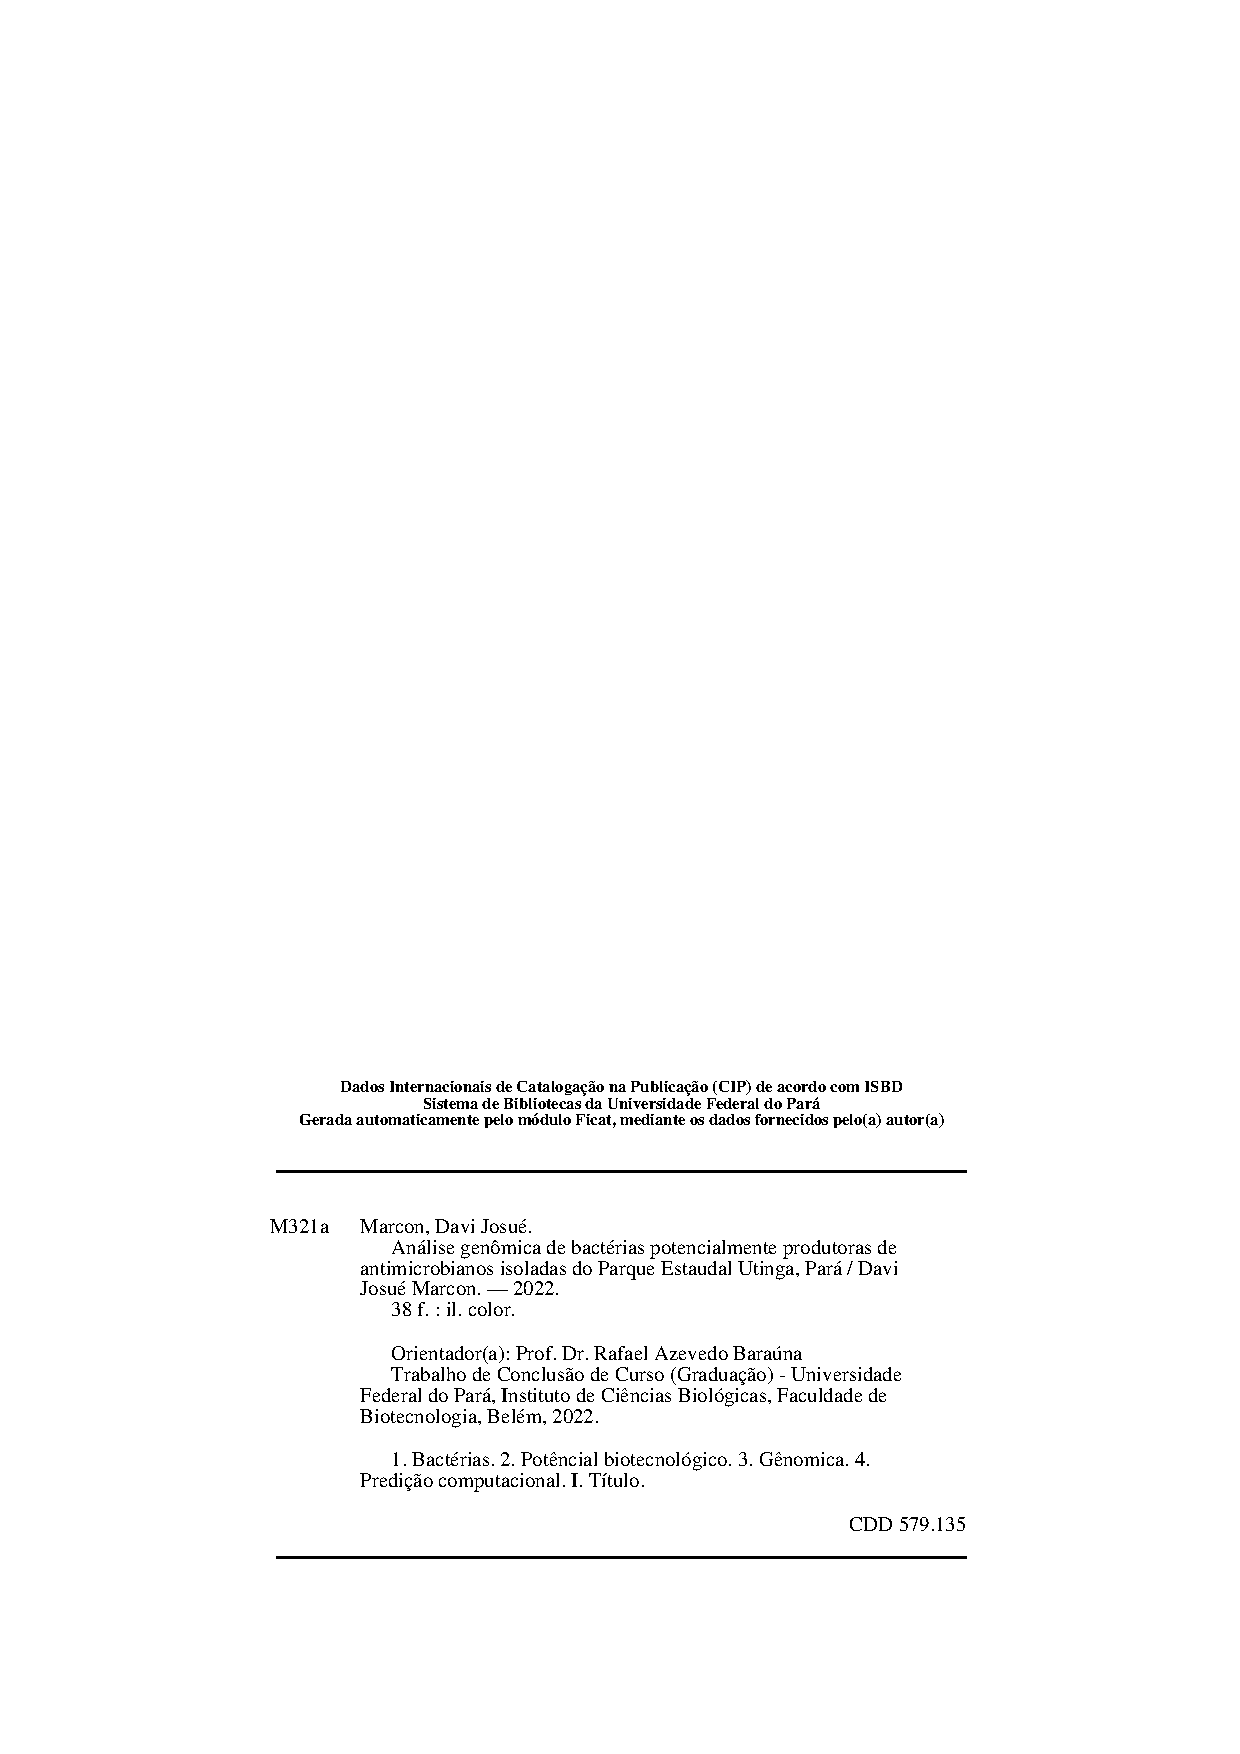
\includepdf{ficha_catalografica.pdf}
\end{fichacatalografica}
% ---

% ---
% Inserir errata
% ---
%\begin{errata}

%Elemento opcional da \citeonline[4.2.1.2]{NBR14724:2011}. Exemplo:

\vspace{\onelineskip}

FERRIGNO, C. R. A. \textbf{Tratamento de neoplasias ósseas apendiculares com
reimplantação de enxerto ósseo autólogo autoclavado associado ao plasma
rico em plaquetas}: estudo crítico na cirurgia de preservação de membro em
cães. 2011. 128 f. Tese (Livre-Docência) - Faculdade de Medicina Veterinária e
Zootecnia, Universidade de São Paulo, São Paulo, 2011.

\begin{table}[htb]
\center
\footnotesize
\begin{tabular}{|p{1.4cm}|p{1cm}|p{3cm}|p{3cm}|}
  \hline
   \textbf{Folha} & \textbf{Linha}  & \textbf{Onde se lê}  & \textbf{Leia-se}  \\
    \hline
    1 & 10 & auto-conclavo & autoconclavo\\
   \hline
\end{tabular}
\end{table}


%\end{errata}
% ---

% ---
% Inserir folha de aprovação
% ---

% Isto é um exemplo de Folha de aprovação, elemento obrigatório da NBR
% 14724/2011 (seção 4.2.1.3). Você pode utilizar este modelo até a aprovação
% do trabalho. Após isso, substitua todo o conteúdo deste arquivo por uma
% imagem da página assinada pela banca com o comando abaixo:
%
% \includepdf{folhadeaprovacao_final.pdf}
%
%\begin{folhadeaprovacao}
%\imprimirfolhadeaprovacao
%\end{folhadeaprovacao}
% ---

% ---
% Dedicatória
% ---
\begin{dedicatoria}

\vspace*{\fill}
   \centering
   \noindent
   \textit{Este trabalho é dedicado a todos aqueles que,\\
   de alguma forma abdicaram de algo e\/ou a si mesmos\\
   pela Ciência.} \vspace*{\fill}


\end{dedicatoria}
% ---

% ---
% Agradecimentos
% ---

\begin{agradecimentos}
Pela orientação e angario de financiamento: Rafael Baraúna, Paula Schneider, Arthur Silva. 

A equipe do Centro de Gênomica e Biologia de Sistemas: Beatriz Lobato, Carolina Miranda, Soraya Andrade,
Silvanira Barbosa. 

Aos desenvolvedores, usuários e contribuintes dos projetos \abnTeX, \LaTeX, nextflow, powershell, 
prokka, antismash, blast, fastq, multiqc, armfinder, ragout, busco, kraken, artemis e demais projetos
associados.

Alexandra Elbakyan e ao(s) fundador(es) da Genesis Library.

Aos meus pais e meus irmãos: Fábio, Silvane, Israel, Giulia e Laura Marcon.

Aos meus amigos e colegas: Cayo Uchôa, Tiago Moura, Gustavo Marques, Joaquim Neto, Thiago Cordeiro, Naiana Ribeiro, 
Valéria Silva, Giovane Pinheiro, Gabriela Campestrini, Wictoria Dias, Aline Castro, Mayanne Farias, Amanda Oliveira, 
Letícia Lago, José Lucas, Iago Blanco, Isabel Montoril, Gabrielly Andrade, Mayza Miranda,
Beatriz Moura, Beatriz Campos. 

A minha namorada: Clara Feitosa.

Colaboradores externos a minha formação: Emilyn Conceição, Abhinav Sharma, Marília Lima, Karla Lima, Alex Souza, Robert Petit III.

Aos professores: Luciana Xavier, Agenor Valadares, Rommel Jucá, Moysés Miranda, Adriana Folador,
Bruno Duarte, Ricardo de Deus e Alejandro Prado.

Pela estrutura: Universidade Federal do Pará, Centro de Gênomica e Biologia de Sistemas, ENGBIO.

As fontes de financiamento: CAPES, CNPQ, FAPESPA, UFPA.


Nenhum trabalho é feito sozinho.


Obrigado.

\end{agradecimentos}


% ---

% ---
% Epígrafe
% ---
\begin{epigrafe}
    
\vspace*{\fill}
	\begin{flushright}
		% Consistency is contrary to nature, contrary to life.
        % The only completely consistent people are the dead.” 
		\textit{``A consistência é contrária à natureza,
		\\ contrária à vida. As únicas pessoas completamente 
		\\ consistentes são os mortos.
        \\são os mortos.''\\
		(Aldous Huxley -  Do What You Will)}
	\end{flushright}


\end{epigrafe}
% ---

% ---
% RESUMOS
% ---

\setlength{\absparsep}{18pt} % ajusta o espaçamento dos parágrafos do resumo
\begin{resumo}

A mineração genômica permite predizer a capacidade de microrganismos produzirem
metabólitos de interesse biotecnológico. A partir do sequenciamento de duas cepas
bacterianas $($\textit{Rhodococcus sp.} e \textit{Brevibacillus brevis} $)$, foi 
possível montar seu genoma utilizando a ferramenta SPADES, predizer os genes nos
genomas utilizando a ferramenta PROKKA e predizer a produção de Metabólitos 
secundários usando o ANTI-SMASH.  Como principais resultados obtivemos que a cepa
de \textit{Rhodococcus sp.}, observamos a presença de 16 clusters ainda sem a função definida.
A amostra \textit{Brevibacillus brevis} apresentou 15 clusters sendo 3 com função predita
para atividade antimicrobiana. A técnica de mineração genômica, permitiu prospectar informações
a respeito da produção de metabóltios, com isso foi possível avaliar o potencial biotecnológico
desses organismos com técnicas independentes de cultivo.

\vspace{\onelineskip}
\noindent 
\textbf{Palavras-chave}: bactérias, potencial biotecnológico, genômica, predição computacional

\end{resumo}

% resumo em inglês
\begin{resumo}[Abstract]
 \begin{otherlanguage*}{english}
   This is the english abstract.
   \vspace{\onelineskip}
   \noindent 
   \textbf{Keywords}: bacterias, biotechnological potential, genomic, computational prediction.
 \end{otherlanguage*}
\end{resumo}

% resumo em francês 
%\begin{resumo}[Résumé]
% \begin{otherlanguage*}{french}
%    Il s'agit d'un résumé en français.
% 
%   \textbf{Mots-clés}: latex. abntex. publication de textes.
% \end{otherlanguage*}
%\end{resumo}

% resumo em espanhol
%\begin{resumo}[Resumen]
% \begin{otherlanguage*}{spanish}
%   Este es el resumen en español.
%  
%   \textbf{Palabras clave}: latex. abntex. publicación de textos.
% \end{otherlanguage*}
%\end{resumo}


% ---
% Listas de siglas, tabelas e simbolos
% ---

% ---
% inserir lista de ilustrações
% ---
\pdfbookmark[0]{\listfigurename}{lof}
\listoffigures*
\cleardoublepage
% ---

% ---
% inserir lista de tabelas
% ---
\pdfbookmark[0]{\listtablename}{lot}
\listoftables*
\cleardoublepage
% ---

% ---
% inserir lista de abreviaturas e siglas
% ---
\begin{siglas}
	\item[BGC] \textit{Biosyntetic Genes Cluster } - Cluster de Genes Biossintéticos
  \item[AMP] \textit{Antimicrobial Peptides} - Peptídeos Antimicrobianos
  \item[MIB] Microrganismos de Interesse Biotecnológico
  \item[NCBI] \textit{National Center of Biotechnology Information}
  \item[DNA] \textit{Deoxyribonucleic acid} - Ácido Desoxirribonucleico
  \item[RNA] \textit{Ribonucleic acid} - Ácido ribonucleico
  \item[ARG] \textit{Antibiotic Resistance Gene} - Gene de resistência a antibiótico
\end{siglas}
% ---


% ---
% inserir o sumario
% ---
\pdfbookmark[0]{\contentsname}{toc}
\tableofcontents*
\cleardoublepage
% ----------------------------------------------------------
% ELEMENTOS TEXTUAIS
% ----------------------------------------------------------
\textual
\pagestyle{simple}
% ----------------------------------------------------------
% Introdução
% ----------------------------------------------------------
\section{Introdução}
\label{cap:introducao}

\subsection{Contexto}


- Necessidade de novos Compostos

- Uso de Biotecnologia para solução de problemas industriais
A biotecnologia 

Os ambientes amazônicos são um reservatório de biodiversidade muito importantes,
a riqueza de espécies e o uso da biotecnologia como ferramenta para a solução de problemas relacionados
a saúde humana e animal, indutriais(XXX). Seu patrimônio genético é fonte interessante para o
desenvolvimento sustentável baseado no uso de tecnologia de ponta para a formulação de novas tecnologias.
Microorganismos do solo amazônico podem ser a fonte de novos fármacos para doenças já conhecidas,
a cura para doenças emergentes, biofábricas para novos procesos industriais e biorremediadores
de impactos ambientais.

\subsection{Justificativa}
Bactérias ambientais são interessantes alvos para a descoberta de compostos
de relevância biotecnológica, especialmente como solução para os crescentes níveis
de resistência a antimicrobianos encontrados em microorganismos patogênicos.
A caracterização genômica e prospecção de genes de interesse desses microorganismos,
especialmente do ambiente amazônico, são passos importantes
em busca de compostos de potencial farmacológico e industrial.

\chapter{Objetivos}

\subsection{Objetivo Geral}

Predizer o potencial biotecnológico de bactérias ambientais utilizando 
ferramentas \textit{in silico} 

\subsection{Objetivos Específicos}
\begin{enumerate}
    \item Caracterizar os organismos sequênciados utilizando seus genomas
    \item Predizer as características metabólicas dos organismos
    \item Categorizar os microorganismos quanto a capacidade de produção de compostos de interesse biotécnológico
\end{enumerate}






% ----------------------------------------------------------
% Referenciais Teóricos
% ----------------------------------------------------------
\chapter{Referenciais Teóricos}\label{cap:referenciais_teoricos}

\section{Metabolitos secundários}

O metabolismo celular bacteriano é o conjunto de processos bioquímicos anabólicos e catabólicos no qual
as células bacterianas produzem novos substâncias a partir de substrato ou outras substâncias, os produtos
dessas reações são conhecidos como metabólitos. Podendo ser classificados como primários ou secundários, 
sendo os primários o conjunto de substâncias essenciais para a sobrevivência do organismo, relacionadas 
a produção de energia e as funções vitais da célula, já os secundários não estão relacionados a sobrevivência
da célula, mas sim sua perpetuação no ambiente utilizando estratégias de resistência a situações adversas \cite{gokulan2014}.  

A maquinaria responsável pela produção desses compostos, normalmente está relacionada a aglomerados 
de genes biossintéticos (\textit{Biosyntetic Genes Cluster - BGC}) que são dois ou mais genes 
agrupados codificam a via biosintética para a produção de um metabólito, sendo capazes de produzir compostos
das seguintes classes: alcalóides, carboidratos, esteroídes, lipídeos, peptídeos (com ou sem modificações pós-traducionais), policetídeos e
terpenóides \cite{medema2015}. 

Esses metabólitos possuem uma diversa gama de funções, seja como metodologia de "guerra
química" com outros microorganismos, mediadores de atividade mutualística entre espécies ou
simbiose química \cite{obrien2011}. Apesar de não serem considerados essenciais para a vida 
desses organismos \cite{demain2009} são de grande importância para sua dispersão e adaptação
em ambientes hostis e excassos de nutrientes. 

É importante ressaltar que a produção de metabólitos de ação antimicrobiana, está relacionada
com a resistência a antimicrobianos, uma vez que, microorganismos produtores de substâncias antimicrobianas
precisam resistir a sua ação de forma a evitar o suicídio causado pelas suas próprias substâncias \cite{cundliffe2010avoidance}.

\section{Resistência a antimicrobianos}
Bactérias possuem diversos mecanismos para proteção contra agentes antimicrobianos como: desativação do fármaco, 
mutação no sítio de ligação do fármaco, expressão de bombas de efluxo e desvios metabólicos. Esses mecanismos, podem
estar associados a elementos genéticos móveis permitindo a transferência entre indivíduos da mesma espécie ou não \cite[p. 150]{Madigan2021}.

A resistência a antibióticos é um problema emergente que está associado a mortalidade em patógenos bacterianos e sua solução
é complexa e permeia a necessidade de políticas públicas, vigilância e controle do uso de antibióticos, medidas de prevenção 
e o desenvolvimento de novas opções de tratamento \cite{frieri2017antibiotic}.  
%Tu não queres escrever mais sobre resistência não? Sei lá, 
% sobre como novas moléculas podem driblar isso… 
% análise genômica das bactérias permite a modulação de expressão etc


\section{Actinomicetos}

Actinomicetos são um filo de microorganismos gram-positivos de alto conteúdo
guanina e citosina que contém as classes: Acidimicrobiia, Actinobacteria, 
Coriobacteriia, Nitriliruptoria, Rubrobacteria, e Thermoleophilia\cite{yadav2018}.
Dentre suas principais caracteristicas podemos ressaltar a presença de micélios
e a produção de hifas filamentosas \cite{chater2016}. Sua dispersão ambiental é enorme
e já foram isolados de ambientes diversos como: lagos salinos, mar profundo e solo \cite{flores2021,felicio2021,sapkota2020}.
Além da simbose com animais, fungos, insetos, línquens e plantas \cite{hei2021,van2017}.
A capacidade de se adaptar a diversos ambientes está intimamente relacionada com a capacidade
de produzir substâncias bioativas com funções igualmente diversas  \cite{van2020}

Essas bactérias foram uma fonte importante para o desenvolvimento de compostos de funções
diversas como: antibactericidas, antifungicos, antihelminticos, antitumorais, anticancererigenos,
antinflamatorios, antivirais, imunossupressores, inseticidas e herbicidas \cite{demain2009,jose2021}. 
64\% dos antibióticos derivados de produtos naturais foram obtidos a partir de actinomicetos filamentosos,
especialmente durante a era de ouro dos antibióticos (1940-1960) sendo 20 utilizados clinicamente \cite{hutchings2019} .
Segundo \citeonline{genilloud2017}, continuam sendo uma fonte relevante
para o isolamento de caracterização de compostos de interesse biotecnológicos, e com o
emprego de metodologias modernas de investigação podem continuar a fornecer
substâncias relevantes para mercado. 


\subsection{\textit{Rhodococcus}}
O gênero \textit{Rhodococcus} contem actinomicetos de diversidade genômica e fisiológica,
contendo alguns membros patógenos para humanos, animais e plantas. Sua importância biotecnológica
é encontrada principalmente por conter algumas cepas com capacidade de degradar compostos orgânicos.
Devido seu grande tamanho gênomico (8.5-10Mb) esses microorganismos possuem grande liberdade
para modifcar seu genoma com recombinações, translocações e inserções, contendo diversas vias catabólicas,
e mantendo multiplas funções metabólicas \cite{cappelletti2019}.

\textit{Rhodococcus} são os microorganismos mais adequados para o desenvolvimento de
tecnologias de remediação de ambientes por serem capazes de degradar poluentes persistentes e por
terem sido isolados de ambientes contaminados com hidrocarbonetos 
(inclusive em forma gasosa)\cite{kuyukina2019}. Sua resitência a intemperes como frio, calor, acidez,
salinidade, pode ser explorada para o desenvolvimentode biorremediadores de derramamento de derivados
de petróleo.

Além da capacidade de remediação biológica, podemos ressaltar o potencial de produção de diversas moléculas
como: biosulfactantes, biofloculantes, carotenoides, ácidos graxos poli-insaturados, poli-hidroxi-alcalóides e
triacil-glicerois \cite{cappelletti2020}. Essas estruturas especialmente as mais complexas como os
Carotenoides e os Ácidos graxos Poli-Insaturados são de grande interesse industrial pois sua síntese 
é complexa e custosa, o uso de microorganismos pode facilitar e reduzir os custos nesses processos.

Dentre as possibilidades para o uso biotecnológico de \textit{Rhodococcus} temos o uso como biofábricas 
para óleo, biocatálise em processos industriais e valorização de rejeitos \cite{alvarez2021,krivoruchko2019,anthony2019,chatterjee2020}.

\section{\textit{Brevibacillus brevis}}
\textit{Brevibacillus} (anteriormente \textit{Bacillus brevis}) é um gênero com grande potêncial para uso organismo para uso como organismo de expressão heteróloga
por ter crescimento rápido, baixa produção de proteases extracelulares e boa eficiência de transformação
por eletroporação, além disso diversos membros do gênero produzem substâncias com atividades 
larvicidas e antimicrobianas e tem grande importância agroecológica por sua relação mutualística
com plantas promovendo seu crescimento, protegendo de doenças e removendo metais pesados do solo
\cite{panda2014brevibacillus,ray2020brevibacillus}.  

\citeonline{yao2020available} ressaltam  capacidade prolífica de \textit{Brevibacillus} para expressão heteróloga
especialmente sua capacidade de produzir moléculas com eficiência ao ser mediada por promotores endógenos
com repetição em tandem e peptídeos sinal, sugerindo a importância do uso de estratégias eficazes de otimização do hospedeiro, do vetor,
do processo fermentativo e o estudo detalhado dos promotores do gênero para melhoria desse modelo.

Exemplos importantes de metabólitos obtidos de \textit{Brevibacillus} temos os peptídeos antimicrobianos (AMP),
sendo esses classificados pela sua síntese ribossomal ou não, tendo diversos usos como o biocontrole em plantas, preservantes
para alimentos em prateleiras\cite{yang2018antimicrobial}. Além dos AMPS podemos citar a probdigiosina com atividade algicida e compostos ainda não
elucidados com grande atividade antiproliferativa \cite{zhang2022transcriptome,arumugam2018isolation}.
Além dos metabólitos, algumas vias bioquímicas dos \textit{Brevibacillus} são interessantes pela capacidade de
degradar Ácido Polilático (plástico biodegradável), a síntese de exopolissacarídeos e a 
biodegradação de polietileno \cite{yu2022comparison,yildiz2015genomic,hadad2005biodegradation,ali2022screening}.

A espécie \textit{Brevibacillus Brevis} contém espécies majoritariamente mesofílicas, e
sua distinção é baseada em similaridade genômica, sondagem molecular e análises 
quimiotaxonômicas \cite{ray2020brevibacillus}.  

\section{Estudo MIB's}
%- Nesse tópico podes iniciar abordando a questão do desinteresse em prospectar novas moléculas por conta dos processos padrões serem custosos, e que isso levou ao desinteresse da industria. 
%- No  entanto com o advento de novas tecnologias (escreve um pouco de cada), estão sendo retomadas a exploração pelo potencial biossintetico de microrg.
%- Que antes do sequenciamento do genoma pouco se sabia sobre o potencial biossintético das bactérias
%
Em 2012 \citeonline{berdy2012thoughts} comentou a respeito do declínio no desenvolvimento de novos
fármacos, sendo eles resultantes de falhas humanas devido ao uso irresposável de medicamentos,
falhas científicas devido a limitações técnicas e ambientes econômicos de regulação custosos e estritos
que limitam o desenvolvimento de novos medicamentos.
Após o fim da era de ouro dos antibióticos, um decréscimo dramático foi observado no nos níveis
de descoberta de novos fármacos, apesar disso, o desenvolvimento nas áreas de espectometria de massas,
metabolômica, genômica e transcriptômica além do baixo custo para o sequenciamento de um genoma são
ferramentas importantes para o direcionamento no desenvolvimento de novos compostos derivados de produtos naturais \cite{katz2016natural}. 

O uso de ferramentas computacionais para a mineração 
de dados e predição de informações a partir de genomas é uma estratégia promissora por ser
eficiente economica e laborosamente, e podem servir de estratégias guiadoras para o uso de outras 
ferramentas \cite{adamek2017mining}. \citeonline{trivella2018tripod} propõe o uso de um tripé para a identificação de novos produtos
naturais derivados de bactérias, sendo estes: o uso de mineração genômica, a manipulação de condições
de cultivo para eliciação da expressão de genes e a metabolomica baseada em espectometria de massa. Com
essas ferramentas, os autores acreditam que a integração da genômica com técnicas de obtenção e purificação
de metabólitos serão as bases para o desenvolvimento de novos produtos farmacológicos pelos próximos anos.

\citeonline{ramirez2022} ressalta a relevância de bactérias para a descoberta de importantes
fármacos e propõe que organismos de fontes não convencionais como cavernas, fontes termais,
areas de alta salinidade, solos áridos, oceanos e mares continuem sendo estudados especialmente
com tecnologias como metagnômica e mineração genômica pois podem ter um papel importante no 
combate de possíveis surtos de doenças como a SARS-COV2 e epidemias causadas por bactérias resistentes.


Em condições laboratoriais, muitos genes relacionados a síntese de
compostos bioativos são silenciados, limitando a produção a produção desses produtos, propondo
que o uso de eliciadores é necessário para expressão dos genes relacionados a produção desses 
compostos\cite{rutledge2015}. \citeonline{felicio2021} propõe o uma metodologia de eliciação para expressão, purificação
e caracterização desses compostos além de ressaltar que até 45\% dos compostos produzidos por
microorganismos são metabólitos secundários eliciados.

Através de Tecnologias modernas como a ferramenta ANTI-SMASH \cite{antismash} é possível predizer
genes putativos e \textit{clusters} gênicos relacionados a produção de metabólitos secundários
e de síntese ribossomal. Essa tecnologia de mineração \textit{in silico} permite prever redes
metabólicas e possíveis promotores da expressão desses compostos, principalmente por utilizar
bancos de dados produzidos a partir de outras ferramentas como BAGEL, NORINE e CLUSEAN \cite{bagel2,bagel3,norine,clusean}.
A incorporação de diversas ferramentas e banco de dados permite uma análise robusta 
e completa utilizando tecnologias do estado da arte da biologia computacional.

% ----------------------------------------------------------
% Metodologia
% ----------------------------------------------------------
\chapter{Metodologia}
\section{Seleção de amostras}
Foram selecionados 4 microorganismos de espécies diferentes do banco de amostras ambientais provenientes
do parque estadual Utinga - Belém, PA gentilmente disponibilizadas pelo Centro de Gênomica e Biologia de Sistemas.
Incluindo três Actinobacterias: \textit{Kitasatospora sp.},\textit{Rhodococcus sp.} e \textit{Streptomyces sp.}
e uma bactéria do filo \textit{Firmicutes}: \textit{Brevibacillus brevis}.
Essa amostras foram previamente identificadas utilizando sequênciamento do gene de RNA ribossomal 16s
utilizando os primers universais 8F: 5'-AGAGTTTGATCATGGCTCAG-3' e 1492R: 5'-CGGTTACCTTGTTACGACTT-3' com o sequenciador 
ABI Prism 3500 Genetic Analyzer (Applied BioSystems). Posteriormente as espécies foram preditas utilizando
homologia baseada no alinhamento contra o banco de dados de RNA ribossomal do NCBI utilizando a ferramenta
blast.

\section{Extração de DNA}
As amostras foram cultivadas em meio Tryptone Soy Broth (TSB) por 48 horas á 28 graus, e em
seu DNA foi extraído utilizando o kit HiPureA Multi-sample DNA Purification Kit(HI-MEDIA) seguindo as orientações
do fabricante. O DNA foi quantificado usando quantificador Quibit(TODO) e sua intigridade foi 
avaliada por eletroforese em gel de agarose 1\% complementado com brometo de estídio 0.5\%.

\section{Sequênciamento e análise genômica}
As bibliotecas foram preparadas utilizando o protocolo do fabricante e sequênciadas no equipamento
Ion GeneStudio S5 Plus (Thermo Fisher)
Após o sequênciamento as amostras foram submetidas ao pipeline Bactopia, o qual filtrou
as leituras, montou e anotou o genoma. Após isso, foram utilizadas as ferramentas do Bactopia 
para análise de resistência, genes patogênicos, genes de produção de compostos, clusters
gênicos e elementos moveis. 
Foram utilizados os softwares GoFeat,Anti-Smash versão 6, BRIG e R para criação de figuras a partir dos dados gerados.

% ----------------------------------------------------------
% Resultados e Discussão
% ----------------------------------------------------------
\chapter{Resultados e Discussão}\label{cap:resultados}

\section{Sequenciamento e controle de qualidade das leituras}
Após o sequenciamento das amostras, foram obtidas 7.8 milhões de leituras de tamanho médio de 
223 pares de base para a amostra ACT016 e 7.4 milhões de leituras com tamanho médio de 222 pares de base
para a amostra ACT094. Após a filtrar as leituras utilizando a ferramenta Trimmomatic, retivemos
6.2 milhões de leituras com tamanho médio 113 pares de base \(perda 21,5\%\) para ACT016 e 6.1 milhões
de leituras com tamanho médio 145 pares de base\(perda de 18,5\%\).

Baseando-se num tamanho de genoma variável de 3 a 10 milhões de bases para \textit{Rhodococcus}, podemos
determinar a cobertura real estimada pela fórmula $C= (L\cdot N)/G $ sendo $C$ a cobertura, $L$ o comprimento
médio das reads e $G$ o tamanho do genoma. A partir disso, obtivemos que a cobertura para a amostra ACT016 Após
filtrar as leituras está entre $70$ e $233,53$ vezes. 
Para a amostra ACT094, consideramos o tamanho do genoma de referência de \textit{Brevibacillus Brevis}(NZ\_LR134338) 
de 6.2 milhões de bases e estimamos a cobertura em aproximadamente $142,66$ vezes.

A qualidade média das sequências pode ser observada a partir dos gráficos gerados pela ferramenta
fastqc:

\begin{figure}[!htb]
	\caption{Gráficos representando a qualidade média das sequências na escala PHRED antes (a esquerda) e depois (a direita) de filtra-las}
	\label{fig:fastqc_antes}
	\centering
	\begin{minipage}{.45\linewidth}
		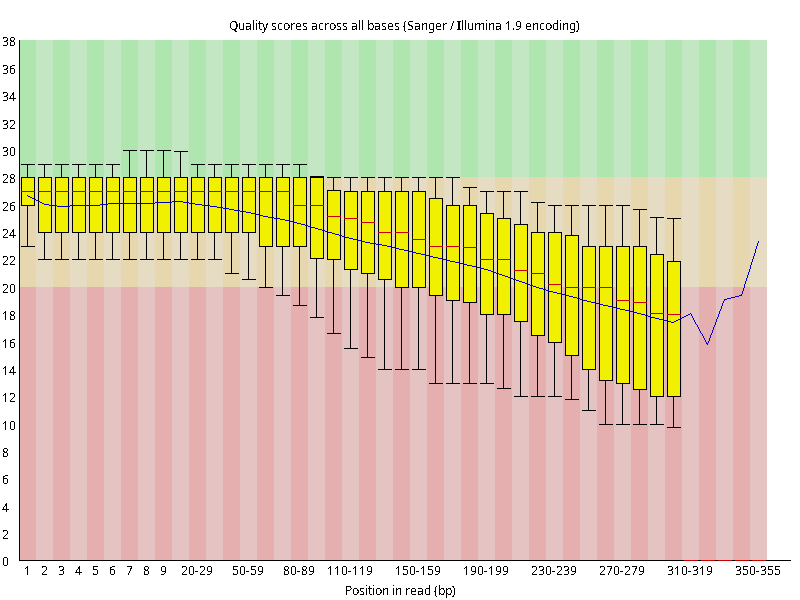
\includegraphics[width=\linewidth]{imagens/read\_qc/002.png}
	  \end{minipage}
	  \hspace{.05\linewidth}
	  \begin{minipage}{.45\linewidth}
		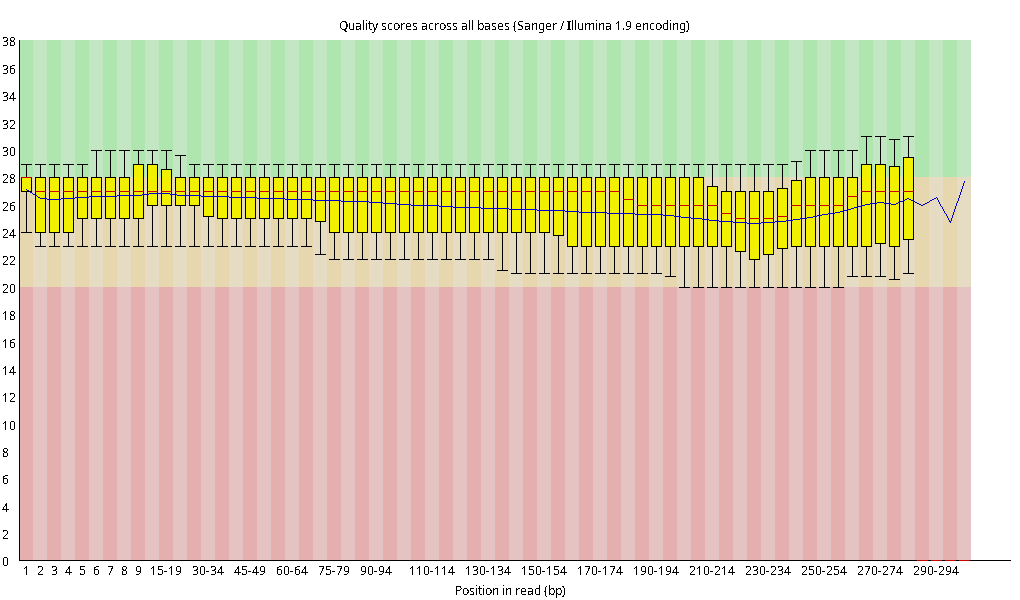
\includegraphics[width=\linewidth]{imagens/read\_qc/002trimmed.png}
	  \end{minipage}
    \begin{small}\textbf{Fonte: O Autor (2022)}\end{small}
\end{figure}

% ----------------------------------------------------------
% Considerações Finais
% ----------------------------------------------------------
\chapter{Conclusão}
\label{conclusao}

%Quais clusters foram encontrados? 
%Existe indicação de clusters pouco estudados nos genomas?
%a montagem ds genomas apresentou parâmetros satisfatórios (N50, CG, número de genes, tamanho…)?
% O Parque Estadual para ser uma boa fonte de micro-organismos com potencial biotecnológico?
% Responder todas estas perguntas ajuda a preparar uma conclusão melhor.

% podes inserir a importância da análise genômica como um guia pra prospecção,
% por meio dos elicitores, visto que alguns elicitores induzem especificamente algumas moléculas.
%


Como resultados desse trabalho obtivemos a montagem de 2 novos genomas a fim de depositar no GenBank. Além de ter descrito o potêncial biotecnológico da amostra 094
através de ferramentas \textit{in silico}, abrindo espaço para metodologias confirmatórias para
estudo detalhado dos metabólitos desse microrganismo. A cepa da amostra 016 apesar de não tem apresentado
clusters identificados ainda deve ser estudada detalhadamente, haja vista que seus metabólitos não puderam
ser identificados mesmo ao utilizar os maiores bancos de dados de \textit{clusters} produtores de produtos naturais disponíveis.

O uso das metodologias \textit{in silico} permite a análise detalhada desses organismos, e através desses genomas
outras perguntas ainda  podem ser respondidas como a presença de ilhas de patogenicidade e genes de virulência
além da relação entre esses microrganismos e outros da mesma espécie já descritos anteriormente.

A confirmação da produção de substâncias antimicrobianas será realizada pela equipe do centro de genômica
e Biologia de Sistemas para posterior purificação e descrição de sua estrutura.
% ----------------------------------------------------------
% ELEMENTOS PÓS-TEXTUAIS
% ----------------------------------------------------------
\postextual
% ----------------------------------------------------------

% ----------------------------------------------------------
% Referências bibliográficas
% ----------------------------------------------------------
\bibliography{bibliografia}
% ---


% ----------------------------------------------------------
% Apêndices
% ----------------------------------------------------------

% ---
% Inicia os apêndices
% ---
%\begin{apendicesenv}
	
	% Imprime uma página indicando o início dos apêndices
%	\partapendices
	
% ----------------------------------------------------------
%\chapter{Quisque libero justo}
% ----------------------------------------------------------

%\lipsum[50]

% ----------------------------------------------------------
%\chapter{Nullam elementum urna}
% ----------------------------------------------------------
%\lipsum[55-57]
	
%\end{apendicesenv}
% ---

% ----------------------------------------------------------
% Anexos
% ----------------------------------------------------------

% ---
% Inicia os anexos
% ---
\begin{anexosenv}
	
	% Imprime uma página indicando o início dos anexos
	\partanexos
    \addtocontents{toc}{\protect\setcounter{tocdepth}{0}}
	\setcounter{chapter}{1}
    \section{Resultados importantes durante a graduação}
    % ---
    \subsection{Artigos em co-autoria}
	\includegraphics*[width=0.8\linewidth]{imagens/artigo.png}
    \subsection{Prêmio conferido pelo Comitê internacional de Microbiologia de alimentos e higiene pela 3\textsuperscript{\underline{a}} melhor apresentação no 30 \textsuperscript{\underline{o}} Congresso Brasileiro de Microbiologia}
	
	\includegraphics*[width=0.7\linewidth]{imagens/premio.png}
	
    %\chapter{Cras non urna sed}
    % ---

    %\lipsum[31]

    % ---
    %\chapter{Fusce facilisis lacinia dui}
    % ---

    %\lipsum[32]
	
\end{anexosenv}

\end{document}
